\chapter{Versuchsaufbau und -durchf�hrung}
\begin{figure}[ht]
    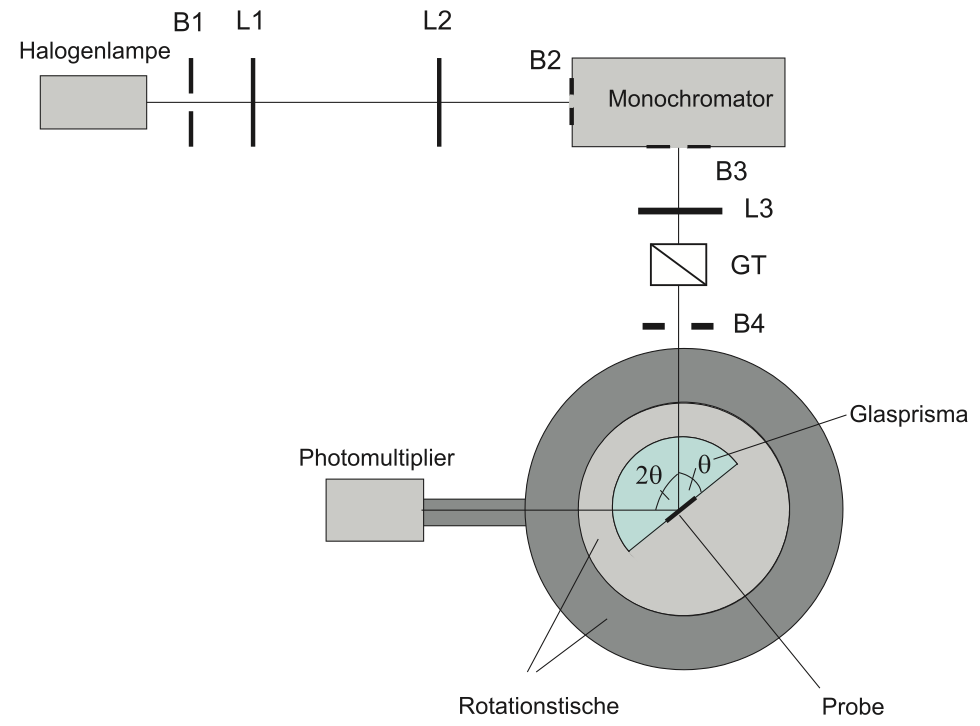
\includegraphics[width=1\textwidth]{op-aufbau.png}
	\caption{Aufbau zur Untersuchung der Oberfl�chenplasmonen}
	\label{fig:opaufbau}
\end{figure}
In diesem Versuch m�chten wir eine Probe mit $p$-polarisiertem monochromatischem
Licht bei variierendem Winkel bestrahlen und dabei den Aufbau so konstruieren,
dass die Wellenl�nge des Lichtes als Parameter sich auch leicht �ndern l�sst. 

Dazu verwenden wir eine Halogenlampe, dessen Licht wir durch eine Blende und
zwei Linsen in einen Monochromator lenken. Die Lampe emittiert ein weites,
kontinuierliches Spektrum an Licht. Im Monochromator wird das Licht in einem 
frequenzabh�ngigen Winkel an einem Gitter gebeugt und durch einen Spalt geschickt.

Das Licht wird dann polarisiert und trifft auf das Glasprisma und die Probe,
wo es die Plasmonen anregen soll. Ein Teil des Lichtes wird auf einen Photomultiplier
reflektiert, wo seine Intensit�t gemessen wird. 

Die Probe ist zusammen mit dem Glasprisma und dem Photomultiplier auf einem
Rotationstisch befestigt. Diesen kann man manuell oder motorisiert bedienen
und damit den Winkel, mit dem das Licht auf die Probe und in den Multiplier reflektiert wird,
abfahren.

Bevor wir mit der eigentlichen Untersuchung der Oberfl�chenplasmonen starten k�nnen,
m�ssen wir zuerst den Winkel des Rotationstisches kalibrieren.
Dazu nutzen wir den Effekt der Totalreflexion aus. Wir konstruieren den Aufbau ohne Probe und messen die Totalreflexion
am �bergang Glasprisma-Luft. Mit Licht einer bestimmten Wellenl�nge fahren wir einen Winkelbereich von ca. (10-50)� ab,
und vergleichen die gemessenen Werte f�r den Totalreflexionswinkel mit den Theoretischen.
Die Differenz zwischen den beiden Werten verwenden wir nun als Kalibrierungskonstante $\theta_0$.



\section{Oberfl�chenplasmonen auf einer glatten Probe}

Im ersten Versuchsteil arbeiten wir mit Silber-Proben, die eine vorgegebene
Schichtdicke von 20nm--70nm haben. Im ersten Durchgang arbeiten wir mit Licht
der Wellenl�nge 550 nm und variieren bei festen Schichtdicken den Einfallswinkel
und messen die Reflektivit�t.
Die Schichtdicke l�sst sich daraus berechnen, N�heres dazu ist in der Auswertung zu finden.


Um die Dispersionsrelation der Oberfl�chenplasmonen zu bestimmen, nehmen wir die
Probe mit dem tiefsten Absorptionsprofil und messen erneut die Relfektivit�t f�r verschiedene Winkel.

\section{Oberfl�chenplasmonen auf einer gittermodulierten Probe}

Bei der Untersuchung der gittermodulierten Probe  bestimmen wir zun�chst die Gitterkonstante.
Dazu nutzen wir die Beugung am Gitter aus.
Mit einem Laser bestrahlen wir die Probe unter einem senkrechten Winkel und
messen den Winkel zwischen den Beugungsmaxima 0. und 1. Ordnung.

In der eigentlichen Messung verwenden wir die Gitter-Probe, wobei der �brige Aufbau
bis auf das Glasprisma, das nun nicht ben�tigt wird, gleich bleibt.
Zur Justage der Gitterprobe kann man die Beugungseffekte ausnutzen,
um die Richtung der Gitterperiodizit�t in die Ebene des Aufbaus einzustellen.

Wir w�hlen einen Messbereich von 475nm--625nm f�r die Wellenl�nge und variieren
jeweils wieder den Einfallswinkel und messen die Reflektivit�t.